\documentclass[a4paper,12pt]{report}
\usepackage[toc,page]{appendix}
\usepackage{amsmath}
\usepackage{float}
\usepackage{graphicx}
\usepackage{subfig}
\usepackage{amssymb}
\usepackage{geometry}
\usepackage{setspace}
 \geometry{
 a4paper,
 total={170mm,257mm},
 left=20mm,
 top=20mm,
 }
\usepackage{tikz}
\usepackage{pgfplots}
\usetikzlibrary{shapes, arrows.meta, decorations.pathreplacing, positioning, petri, fit, calc}
\tikzstyle{startstop} = [circle, minimum size=1cm ,text centered, draw=black]
\tikzstyle{neuron} = [circle, minimum size=1cm ,text centered, draw=red, fill=gray!30]
\tikzstyle{process} = [rectangle, minimum width=2cm, minimum height=0.5cm, text centered, text width=3cm, draw=black, fill=blue!30]
\tikzstyle{detail} = [rectangle, minimum width=1.5cm, minimum height=0.5cm, text justified, text width=2.6cm, fill=white!30]
\tikzstyle{largedetail} = [rectangle, minimum width=3cm, minimum height=1cm, text centered, text width=4cm, fill=white!30]
\tikzstyle{box} = [rectangle, minimum width=5cm, minimum height=9cm, text centered, text width=4cm, draw=black, fill=white!30]

\usepackage[utf8]{inputenc}

% Default fixed font does not support bold face
\DeclareFixedFont{\ttb}{T1}{txtt}{bx}{n}{10} % for bold
\DeclareFixedFont{\ttm}{T1}{txtt}{m}{n}{10}  % for normal

% Custom colors
\usepackage{color}
\definecolor{deepblue}{rgb}{0,0,0.5}
\definecolor{deepred}{rgb}{0.6,0,0}
\definecolor{deepgreen}{rgb}{0,0.5,0}

\usepackage{listings}

% Python style for highlighting
\newcommand\pythonstyle{\lstset{
language=Python,
basicstyle=\ttm,
otherkeywords={self},             % Add keywords here
keywordstyle=\ttb\color{deepblue},
emph={MyClass,__init__},          % Custom highlighting
emphstyle=\ttb\color{deepred},    % Custom highlighting style
stringstyle=\color{deepgreen},
frame=tb,                         % Any extra options here
showstringspaces=false            % 
}}


% Python environment
\lstnewenvironment{python}[1][]
{
\pythonstyle
\lstset{#1}
}
{}

% Python for external files
\newcommand\pythonexternal[2][]{{
\pythonstyle
\lstinputlisting[#1]{#2}}}

% Python for inline
\newcommand\pythoninline[1]{{\pythonstyle\lstinline!#1!}}


\begin{document}
\tableofcontents

\title{Neural Networks \\ Non linear hypothesis}
\maketitle
\part{Week 4}
\section{Introduction}

\begin{figure}[H]
\centering
        \includegraphics[totalheight=3 cm]{example.png}
				\caption{Non-linear classification}
\end{figure}
In this example with 2 features, one could use logistic regression with polynomial terms:
\begin{align*}
g(\theta_0 + \theta_1 x_1 + \theta_2 x_2 + \theta_3 x_1 x_2 + \theta_4 x_1 ^2 + \theta_5 x_2 ^2) 
\end{align*}
However, for larger number of features, the number of quadratic features will grow asymptotically. For example in a problem with 100 features ($x_1, ...x_{100}$), if we include all the 2nd order term: $x_1 ^2, x_1 x_2, x_2 ^{2},..$, we will end up with 5000 features (typically the number of quadratic features grow as $n^2 /2$).

\section{Model representation}
\subsection{Single Neuron model : logistic unit}
\begin{figure}[H]
        \centering
        \resizebox {3in} {!} {
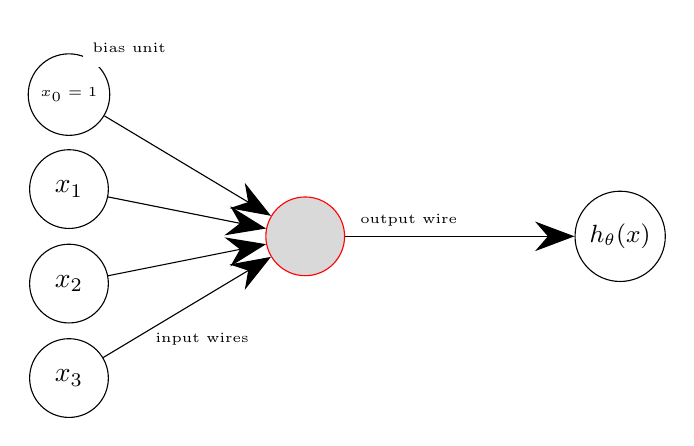
\begin{tikzpicture}[node distance=4cm]
\node (x0) [startstop] {{\tiny $x_0=1$}};
\node (x1) [startstop, below of=x0, xshift=0cm, yshift=2.8cm] {$x_1$};
\node (x2) [startstop, below of=x1, xshift=0cm, yshift=2.8cm] {$x_2$};
\node (x3) [startstop, below of=x2, xshift=0cm, yshift=2.8cm] {$x_3$};
\node (layer3) [neuron, below of=x0, xshift=3cm, yshift=2.2cm] {};
\node (layer4) [startstop, below of=layer3, xshift=4cm, yshift=4cm] {{\small $h_{\theta}(x)$}};
\node (bias) [detail, below of=x0, xshift=1.6cm, yshift=4.6cm] {{\tiny bias unit}};
\node (input) [detail, below of=x3, xshift=2.4cm, yshift=4.5cm] {{\tiny input wires}};
\node (output) [detail, below of=layer3, xshift=2cm, yshift=4.2cm] {{\tiny output wire}};
\draw[-{Stealth[length=5mm]}] (x0) -- (layer3);
\draw[-{Stealth[length=5mm]}] (x1) -- (layer3);
\draw[-{Stealth[length=5mm]}] (x2) -- (layer3);
\draw[-{Stealth[length=5mm]}] (x3) -- (layer3);
\draw[-{Stealth[length=5mm]}] (layer3) -- (layer4);
\end{tikzpicture}
}
\caption{Single neuron with a Sigmoid (logistic) activation function, where $h_{\theta}(x) = \frac{1}{1+\mathrm{e}^{(-\theta^{\mathrm{T}}x)}}$}
\end{figure}
In neural network applications, the parameters $\theta = \left[\begin{smallmatrix} \theta_0 \\ \theta_1 \\ \theta_2 \\ \theta_3 \end{smallmatrix} \right]$ are often called "\textbf{weights}".
Note that the purpose of the activation function is to introduce non-linearity into the network. Non-linear means that the output cannot be reproduce from a linear combination of the inputs. Without a non-linear activation function in the network, a NN, no matter how many layers it had would behave just like a single perceptron. A common activation function used is $tanh$

\subsection{Neuronal model (Diagram representation)}
\begin{figure}[H]
        \centering
        \resizebox {6in} {!} {
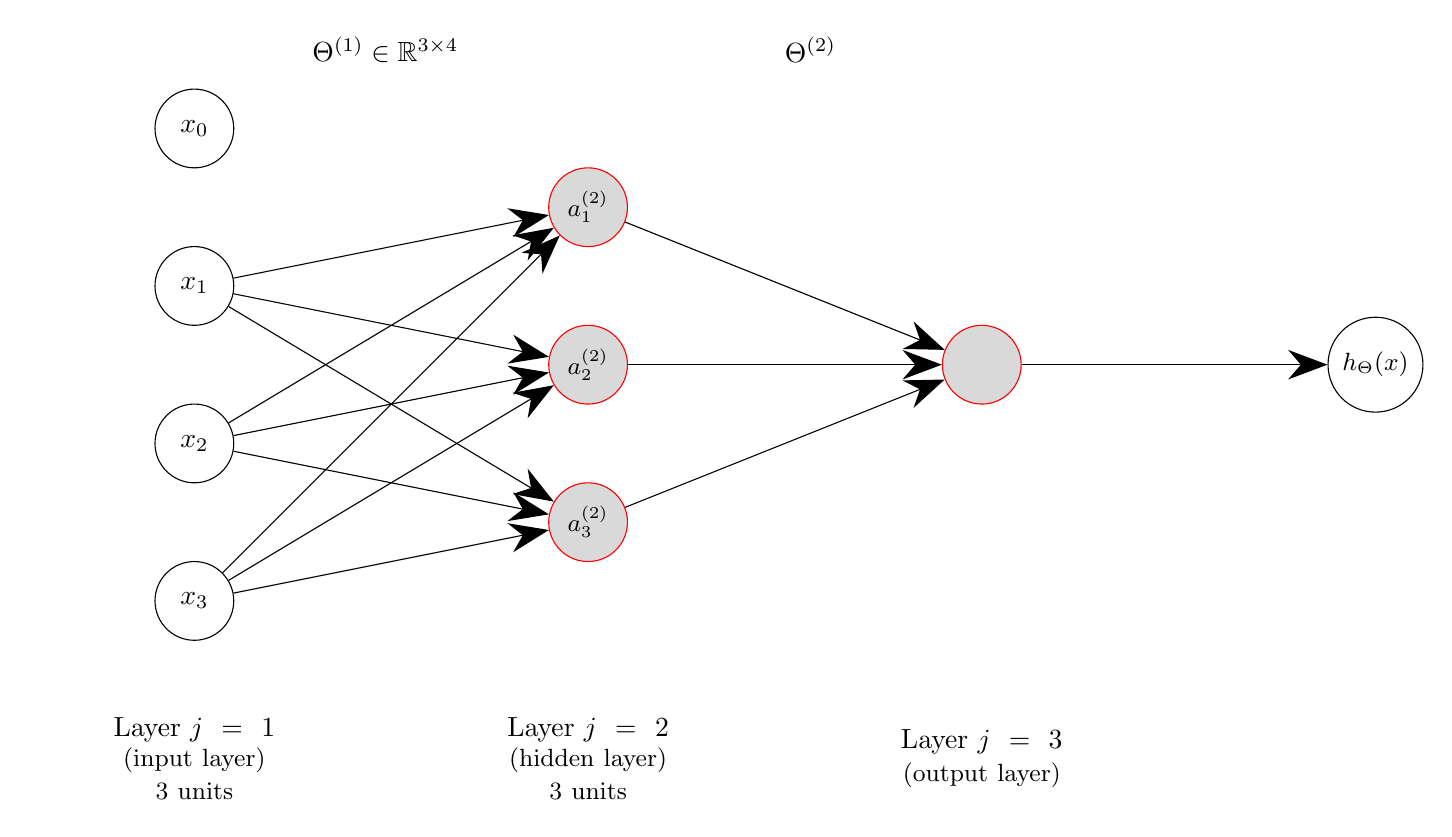
\begin{tikzpicture}[node distance=4cm]
\node (x0) [startstop] {$x_0$};
\node (x1) [startstop, below of=x0, xshift=0cm, yshift=2cm] {$x_1$};
\node (x2) [startstop, below of=x1, xshift=0cm, yshift=2cm] {$x_2$};
\node (x3) [startstop, below of=x2, xshift=0cm, yshift=2cm] {$x_3$};
\node (layer1) [largedetail, below of=x3, xshift=0cm, yshift=2cm] {Layer $j=1$ \\ \small{ (input layer) \\3 units}};
\node (a1) [neuron, below of=x0, xshift=5cm, yshift=3cm] {{\small $a_1 ^{(2)}$}};
\node (a2) [neuron, below of=a1, xshift=0cm, yshift=2cm] {{\small $a_2 ^{(2)}$}};
\node (a3) [neuron, below of=a2, xshift=0cm, yshift=2cm] {{\small $a_3 ^{(2)}$}};
\node (layer2) [largedetail, below of=layer1, xshift=5cm, yshift=4cm] {Layer $j=2$ \\ \small{ (hidden layer) \\3 units}};
\node (layer3) [neuron, below of=a1, xshift=5cm, yshift=2cm] {};
\node (layer3detail) [largedetail, below of=layer3, xshift=0cm, yshift=-1cm] {Layer $j=3$ \\ \small{ (output layer)}};
\node (layer4) [startstop, below of=layer3, xshift=5cm, yshift=4cm] {{\small $h_{\Theta}(x)$}};
\node (theta1) [detail, below of=x0, xshift=2.8cm, yshift=5cm] {$ \Theta ^{(1)} \in \mathbb{R}^{3 \times 4}$};
\node (theta2) [detail, below of=theta1, xshift=6cm, yshift=4cm] {$\Theta ^{(2)}$};

\draw[-{Stealth[length=5mm]}] (x1) -- (a1);
\draw[-{Stealth[length=5mm]}] (x1) -- (a2);
\draw[-{Stealth[length=5mm]}] (x1) -- (a3);
\draw[-{Stealth[length=5mm]}] (x2) -- (a1);
\draw[-{Stealth[length=5mm]}] (x2) -- (a2);
\draw[-{Stealth[length=5mm]}] (x2) -- (a3);
\draw[-{Stealth[length=5mm]}] (x3) -- (a1);
\draw[-{Stealth[length=5mm]}] (x3) -- (a2);
\draw[-{Stealth[length=5mm]}] (x3) -- (a3);
\draw[-{Stealth[length=5mm]}] (a1) -- (layer3);
\draw[-{Stealth[length=5mm]}] (a2) -- (layer3);
\draw[-{Stealth[length=5mm]}] (a3) -- (layer3);
\draw[-{Stealth[length=5mm]}] (layer3) -- (layer4);
\end{tikzpicture}
}
\end{figure}
where $a_i ^{(j)}$ is the activation of unit $i$ in layer $j$. For example $a_1 ^{(2)}$ is the activation (value) of \textbf{unit 1} in \textbf{layer 2}. \\
$\Theta ^{(j)}$ is the matrix of "weights" controlling the function mapping from layer $j$ to layer $(j+1)$.

\subsection{Mathematical representation}
\begin{figure}[H]
        \centering
        \resizebox {5in} {!} {
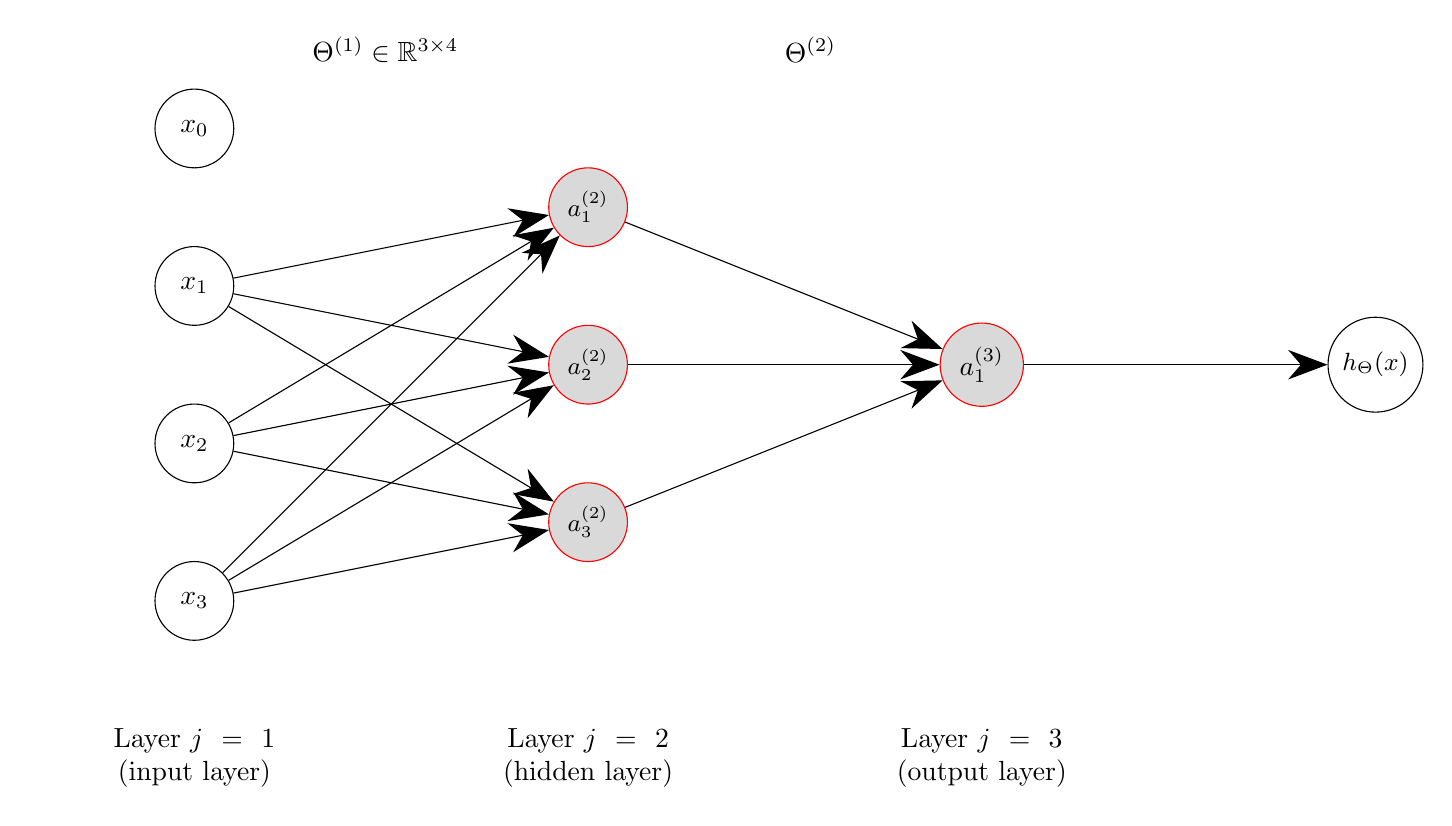
\begin{tikzpicture}[node distance=4cm]
\node (x0) [startstop] {$x_0$};
\node (x1) [startstop, below of=x0, xshift=0cm, yshift=2cm] {$x_1$};
\node (x2) [startstop, below of=x1, xshift=0cm, yshift=2cm] {$x_2$};
\node (x3) [startstop, below of=x2, xshift=0cm, yshift=2cm] {$x_3$};
\node (layer1) [largedetail, below of=x3, xshift=0cm, yshift=2cm] {Layer $j=1$ \\ (input layer)};
\node (a1) [neuron, below of=x0, xshift=5cm, yshift=3cm] {{\small $a_1 ^{(2)}$}};
\node (a2) [neuron, below of=a1, xshift=0cm, yshift=2cm] {{\small $a_2 ^{(2)}$}};
\node (a3) [neuron, below of=a2, xshift=0cm, yshift=2cm] {{\small $a_3 ^{(2)}$}};
\node (layer2) [largedetail, below of=layer1, xshift=5cm, yshift=4cm] {Layer $j=2$ \\ (hidden layer)};
\node (layer3) [neuron, below of=a1, xshift=5cm, yshift=2cm] {$a_1 ^{(3)}$};
\node (layer3detail) [largedetail, below of=layer3, xshift=0cm, yshift=-1cm] {Layer $j=3$ \\ (output layer)};
\node (layer4) [startstop, below of=layer3, xshift=5cm, yshift=4cm] {{\small $h_{\Theta}(x)$}};
\node (theta1) [detail, below of=x0, xshift=2.8cm, yshift=5cm] {$ \Theta ^{(1)} \in \mathbb{R}^{3 \times 4}$};
\node (theta2) [detail, below of=theta1, xshift=6cm, yshift=4cm] {$\Theta ^{(2)}$};

\draw[-{Stealth[length=5mm]}] (x1) -- (a1);
\draw[-{Stealth[length=5mm]}] (x1) -- (a2);
\draw[-{Stealth[length=5mm]}] (x1) -- (a3);
\draw[-{Stealth[length=5mm]}] (x2) -- (a1);
\draw[-{Stealth[length=5mm]}] (x2) -- (a2);
\draw[-{Stealth[length=5mm]}] (x2) -- (a3);
\draw[-{Stealth[length=5mm]}] (x3) -- (a1);
\draw[-{Stealth[length=5mm]}] (x3) -- (a2);
\draw[-{Stealth[length=5mm]}] (x3) -- (a3);
\draw[-{Stealth[length=5mm]}] (a1) -- (layer3);
\draw[-{Stealth[length=5mm]}] (a2) -- (layer3);
\draw[-{Stealth[length=5mm]}] (a3) -- (layer3);
\draw[-{Stealth[length=5mm]}] (layer3) -- (layer4);
\end{tikzpicture}
}
\end{figure}

The activation value of the 3 hidden units of Layer 2 are:
\begin{align*}
\begin{split}
a_1 ^{(2)} & = g\left( \Theta_{1,0} ^{(1)}x_0 +\Theta_{1,1} ^{(1)}x_1 +\Theta_{1,2} ^{(1)}x_2 + \Theta_{1,3} ^{(1)}x_3 \right) \\
a_2 ^{(2)} & = g\left( \Theta_{2,0} ^{(1)}x_0 +\Theta_{2,1} ^{(1)}x_1 +\Theta_{2,2} ^{(1)}x_2 + \Theta_{2,3} ^{(1)}x_3 \right) \\
a_3 ^{(2)} & = g\left( \Theta_{3,0} ^{(1)}x_0 +\Theta_{3,1} ^{(1)}x_1 +\Theta_{3,2} ^{(1)}x_2 + \Theta_{3,3} ^{(1)}x_3 \right) \\
\end{split}
\end{align*}
The activation value of the Layer3 is:

\begin{align*}
h_{\Theta}(x) & = a_1 ^{(3)} \\
              & = g\left( \Theta_{1,0} ^{(2)}a_0 ^{(2)} + \Theta_{1,1} ^{(2)}a_1 ^{(2)} + \Theta_{1,2} ^{(2)}a_2 ^{(2)} + \Theta_{1,3} ^{(2)}a_3 ^{(2)} \right)
\end{align*}

If the network has $s_j$ units in layer $j$ and $s_{j+1}$ units in layer $j+1$, then $\Theta^{(j)}$ will be of dimension $s_{j+1} \times (s_j + 1)$.

\subsection{Vectorized implementation}
\begin{align*}
\begin{split}
a_1 ^{(2)} & = g \underbrace{(\Theta_{1,0} ^{(1)}x_0 +\Theta_{1,1} ^{(1)}x_1 +\Theta_{1,2} ^{(1)}x_2 + \Theta_{1,3} ^{(1)}x_3)}_\text{$z_1 ^{(2)}$} = \Theta^{(1)}x = g(z_1 ^{(2)})\\
a_2 ^{(2)} & = g\underbrace{(\Theta_{2,0} ^{(1)}x_0 +\Theta_{2,1} ^{(1)}x_1 +\Theta_{2,2} ^{(1)}x_2 + \Theta_{2,3} ^{(1)}x_3)}_\text{$z_2 ^{(2)}$} = \Theta^{(2)}x = g(z_2 ^{(2)})\\
a_3 ^{(2)} & = g\underbrace{(\Theta_{3,0} ^{(1)}x_0 +\Theta_{3,1} ^{(1)}x_1 +\Theta_{3,2} ^{(1)}x_2 + \Theta_{3,3} ^{(1)}x_3}_\text{$z_3 ^{(2)}$} = \Theta^{(3)}x = g(z_3 ^{(2)})
\end{split}
\end{align*}
where $z^{(2)}$ is for layer \#2. \\
Remember that the activation applies the sigmoid function element-wise, i.e to each elements of $z^{(2)}$. \\
To make the notation more consistent, we define:
\begin{itemize}
\item $a_0 ^{(2)} = 1$ the bias unit
\item $a^{(1)}=x$ (i.e activation of first layer)
\item $h_{\Theta}(x) = a^{(3)} = g(z^{(3)}$) where $z ^{(3)} = \Theta^{(2)} a^{(2)}$
\end{itemize}

\begin{align*}
\begin{split}
h_{\Theta}(x) & = g(\underbrace{\Theta_{1,0} ^{(2)} + \Theta_{1,1} ^{(2)} a_1 ^{(2)} + \Theta_{1,2} ^{(2)}  a_2 ^{(2)} + \Theta_{1,3} ^{(2)} a_3 ^{(2)}}_{\text{$z^{(3)}$}} ) \\
& = g(z^{(3)}) \\
& = g (\Theta ^{(2)} a^{(2)})
\end{split}
\end{align*}


\begin{figure}[H]
        \centering
        \resizebox {5in} {!} {
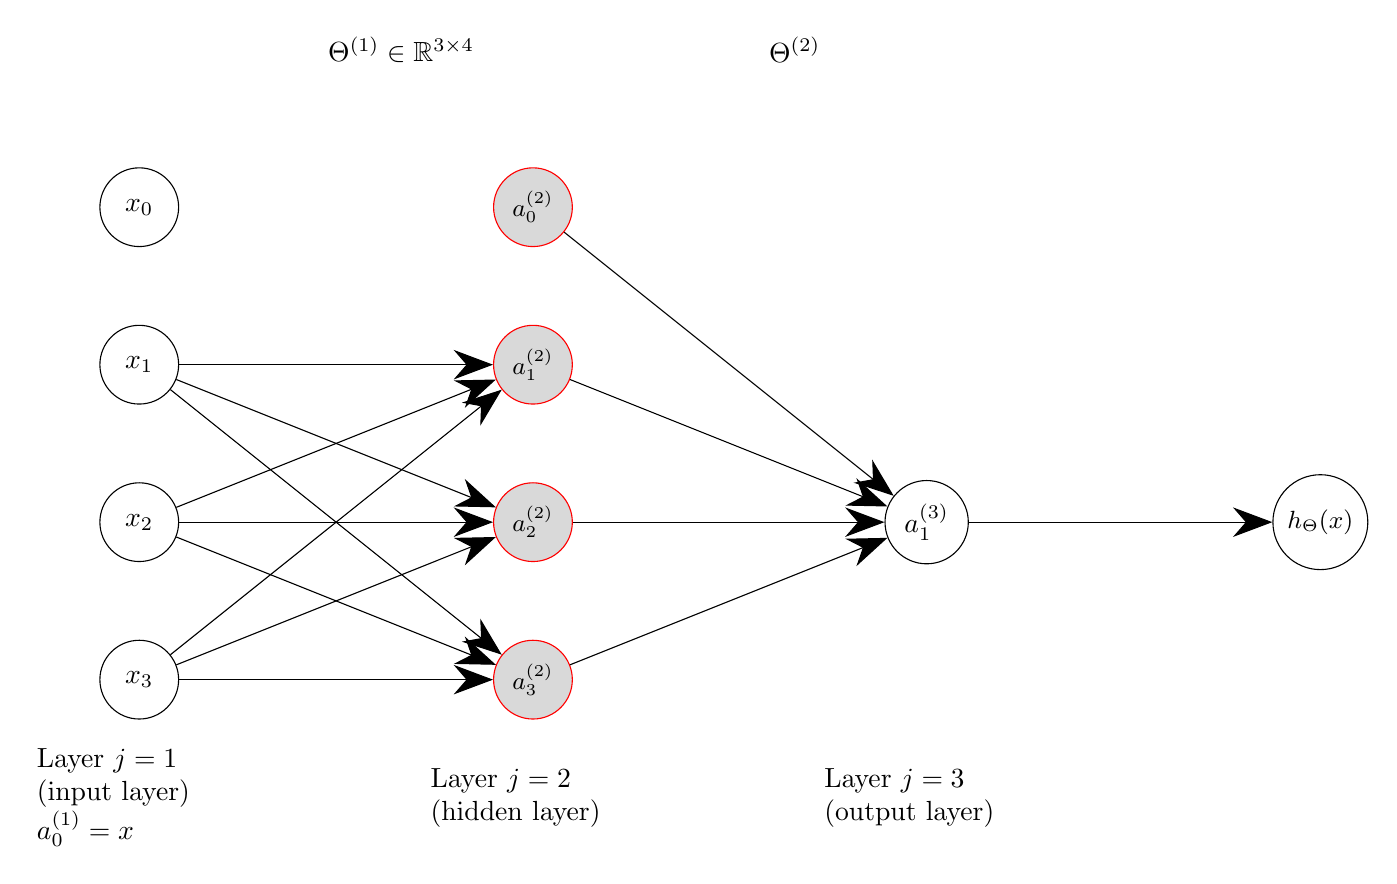
\begin{tikzpicture}[node distance=4cm]
\node (x0) [startstop] {$x_0$};
\node (x1) [startstop, below of=x0, xshift=0cm, yshift=2cm] {$x_1$};
\node (x2) [startstop, below of=x1, xshift=0cm, yshift=2cm] {$x_2$};
\node (x3) [startstop, below of=x2, xshift=0cm, yshift=2cm] {$x_3$};
\node (layer1) [detail, below of=x3, xshift=0cm, yshift=2.5cm] {Layer $j=1$ \\ (input layer) \\ $a_0 ^{(1)} = x$};
\node (a0) [neuron, below of=x0, xshift=5cm, yshift=4cm] {{\small $a_0 ^{(2)}$}};
\node (a1) [neuron, below of=a0, xshift=0cm, yshift=2cm] {{\small $a_1 ^{(2)}$}};
\node (a2) [neuron, below of=a1, xshift=0cm, yshift=2cm] {{\small $a_2 ^{(2)}$}};
\node (a3) [neuron, below of=a2, xshift=0cm, yshift=2cm] {{\small $a_3 ^{(2)}$}};
\node (layer2) [detail, below of=a3, xshift=0cm, yshift=2.5cm] {Layer $j=2$ \\ (hidden layer)};
\node (layer3) [startstop, below of=a1, xshift=5cm, yshift=2cm] {$a_1 ^{(3)}$};
\node (layer3detail) [detail, below of=layer3, xshift=0cm, yshift=0.5cm] {Layer $j=3$ \\ (output layer)};
\node (layer4) [startstop, below of=layer3, xshift=5cm, yshift=4cm] {{\small $h_{\Theta}(x)$}};
\node (theta1) [detail, below of=x0, xshift=3.7cm, yshift=6cm] {$ \Theta ^{(1)} \in \mathbb{R}^{3 \times 4}$};
\node (theta2) [detail, below of=theta1, xshift=5.6cm, yshift=4cm] {$\Theta ^{(2)}$};

\draw[-{Stealth[length=5mm]}] (x1) -- (a1);
\draw[-{Stealth[length=5mm]}] (x1) -- (a2);
\draw[-{Stealth[length=5mm]}] (x1) -- (a3);
\draw[-{Stealth[length=5mm]}] (x2) -- (a1);
\draw[-{Stealth[length=5mm]}] (x2) -- (a2);
\draw[-{Stealth[length=5mm]}] (x2) -- (a3);
\draw[-{Stealth[length=5mm]}] (x3) -- (a1);
\draw[-{Stealth[length=5mm]}] (x3) -- (a2);
\draw[-{Stealth[length=5mm]}] (x3) -- (a3);
\draw[-{Stealth[length=5mm]}] (a1) -- (layer3);
\draw[-{Stealth[length=5mm]}] (a2) -- (layer3);
\draw[-{Stealth[length=5mm]}] (a3) -- (layer3);
\draw[-{Stealth[length=5mm]}] (a0) -- (layer3);
\draw[-{Stealth[length=5mm]}] (layer3) -- (layer4);
\end{tikzpicture}
}
\end{figure}

This method of computing $h_{(\Theta}(x)$ is called \textbf{forward propagation} : we start by calculating the activation of the input $\Rightarrow$ hidden $\Rightarrow$ output layers.

\subsection{what else?}
If the Layer1 is covered up, the diagram is similar to a logistic regression, with $h_{\Theta}(x)$:
\begin{align*}
h_{\Theta}(x) = g(\Theta_0 a_0 + \Theta_1 a_1 + \Theta_2 a_2 + \Theta_3 a_3)
\end{align*}
where the features used are now $a_1, a_2, a_3$ (rather than $x_1, x_2, x_3$), but  computed by the hidden layer.
\newline
\begin{figure}[H]
  \resizebox {4in} {!} {
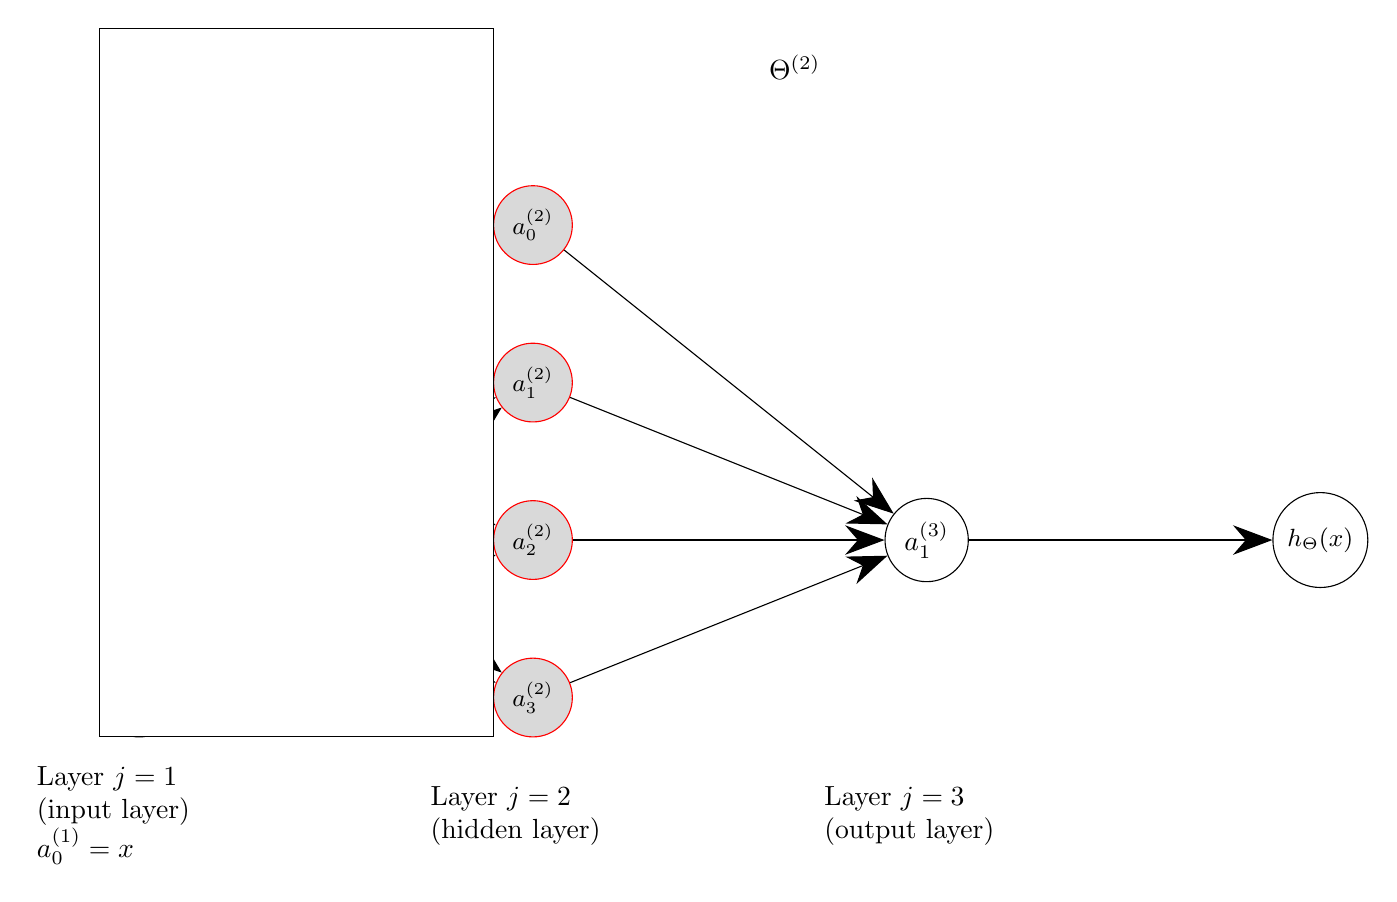
\begin{tikzpicture}[node distance=4cm]
\node (x0) [startstop] {{\tiny $x_0$}};
\node (x1) [startstop, below of=x0, xshift=0cm, yshift=2cm] {{$x_1$}};
\node (x2) [startstop, below of=x1, xshift=0cm, yshift=2cm] {{$x_2$}};
\node (x3) [startstop, below of=x2, xshift=0cm, yshift=2cm] {{$x_3$}};

\node (layer1) [detail, below of=x3, xshift=0cm, yshift=2.5cm] {{Layer $j=1$ \\ (input layer) \\ $a_0 ^{(1)} = x$}};
\node (a0) [neuron, below of=x0, xshift=5cm, yshift=4cm] {{\small $a_0 ^{(2)}$}};
\node (a1) [neuron, below of=a0, xshift=0cm, yshift=2cm] {{\small $a_1 ^{(2)}$}};
\node (a2) [neuron, below of=a1, xshift=0cm, yshift=2cm] {{\small $a_2 ^{(2)}$}};
\node (a3) [neuron, below of=a2, xshift=0cm, yshift=2cm] {{\small $a_3 ^{(2)}$}};
\node (layer2) [detail, below of=a3, xshift=0cm, yshift=2.5cm] {{Layer $j=2$ \\(hidden layer)}};
\node (layer3) [startstop, below of=a1, xshift=5cm, yshift=2cm] {$a_1 ^{(3)}$};
\node (layer3detail) [detail, below of=layer3, xshift=0cm, yshift=0.5cm] {Layer $j=3$ \\(output layer)};
\node (layer4) [startstop, below of=layer3, xshift=5cm, yshift=4cm] {{\small $h_{\Theta}(x)$}};
\node (theta1) [detail, below of=x0, xshift=3.7cm, yshift=6cm] {$ \Theta ^{(1)} \in \mathbb{R}^{3 \times 4}$};
\node (theta2) [detail, below of=theta1, xshift=5.6cm, yshift=4cm] {$\Theta ^{(2)}$};
\draw[-{Stealth[length=5mm]}] (x1) -- (a1);
\draw[-{Stealth[length=5mm]}] (x1) -- (a2);
\draw[-{Stealth[length=5mm]}] (x1) -- (a3);
\draw[-{Stealth[length=5mm]}] (x2) -- (a1);
\draw[-{Stealth[length=5mm]}] (x2) -- (a2);
\draw[-{Stealth[length=5mm]}] (x2) -- (a3);
\draw[-{Stealth[length=5mm]}] (x3) -- (a1);
\draw[-{Stealth[length=5mm]}] (x3) -- (a2);
\draw[-{Stealth[length=5mm]}] (x3) -- (a3);
\draw[-{Stealth[length=5mm]}] (a1) -- (layer3);
\draw[-{Stealth[length=5mm]}] (a2) -- (layer3);
\draw[-{Stealth[length=5mm]}] (a3) -- (layer3);
\draw[-{Stealth[length=5mm]}] (a0) -- (layer3);
\draw[-{Stealth[length=5mm]}] (layer3) -- (layer4);
\node (cover) [box, below of=x0, xshift=2cm, yshift=2cm] {} ;
\end{tikzpicture}
} 
\end{figure}
In the 3 layer neural network, the function mapping from layer 1 to layer 2 is determined by the set of parameters $\Theta_1$, i.e the neural network learned its own features $a_1,a_2,a_3$ to feed into logistic regression.  \\
\\

There can be other \textbf{network architectures}:

\begin{figure}[H]
        \resizebox {5in} {!} {
\begin{tikzpicture}[node distance=4cm]
\node (x1) [startstop, below of=x0, xshift=0cm, yshift=2cm] {$x_1$};
\node (x2) [startstop, below of=x1, xshift=0cm, yshift=2cm] {$x_2$};
\node (x3) [startstop, below of=x2, xshift=0cm, yshift=2cm] {$x_3$};
\node (layer1) [detail, below of=x3, xshift=0cm, yshift=2.5cm] {Layer $j=1$ \\ (input layer)};
\node (a1) [neuron, below of=x0, xshift=4cm, yshift=2cm] {};
\node (a2) [neuron, below of=a1, xshift=0cm, yshift=2cm] {};
\node (a3) [neuron, below of=a2, xshift=0cm, yshift=2cm] {{}};
\node (layer2) [detail, below of=a3, xshift=0cm, yshift=2.5cm] {Layer $j=2$ \\(hidden layer)};
\node (b1) [neuron, below of=x0, xshift=8cm, yshift=1cm] {};
\node (b2) [neuron, below of=b1, xshift=0cm, yshift=2cm] {};
\node (layer3) [detail, below of=layer3, xshift=-1.5cm, yshift=0.5cm] {Layer $j=3$ \\(hidden layer)};
\node (c1) [neuron, below of=b1, xshift=4cm, yshift=3cm] {};
\node (layer4) [detail, below of=layer3, xshift=4cm, yshift=4cm] {Layer $j=4$ \\(output layer)};
\node (h) [startstop, below of=c1, xshift=4cm, yshift=4cm] {{\small $h_{\Theta}(x)$}};
\draw[-{Stealth[length=5mm]}] (x1) -- (a1);
\draw[-{Stealth[length=5mm]}] (x1) -- (a2);
\draw[-{Stealth[length=5mm]}] (x1) -- (a3);
\draw[-{Stealth[length=5mm]}] (x2) -- (a1);
\draw[-{Stealth[length=5mm]}] (x2) -- (a2);
\draw[-{Stealth[length=5mm]}] (x2) -- (a3);
\draw[-{Stealth[length=5mm]}] (x3) -- (a1);
\draw[-{Stealth[length=5mm]}] (x3) -- (a2);
\draw[-{Stealth[length=5mm]}] (x3) -- (a3);
\draw[-{Stealth[length=5mm]}] (a1) -- (b1);
\draw[-{Stealth[length=5mm]}] (a1) -- (b2);
\draw[-{Stealth[length=5mm]}] (a2) -- (b1);
\draw[-{Stealth[length=5mm]}] (a2) -- (b2);
\draw[-{Stealth[length=5mm]}] (a3) -- (b1);
\draw[-{Stealth[length=5mm]}] (a3) -- (b2);
\draw[-{Stealth[length=5mm]}] (b1) -- (c1);
\draw[-{Stealth[length=5mm]}] (b2) -- (c1);
\draw[-{Stealth[length=5mm]}] (c1) -- (h);
\end{tikzpicture}
}
\end{figure}


\section{Non-Linear classification examples }
By the \textbf{universal approximation theorem}, a single hidden layer network with a finite number of neurons can be trained to approximate an arbitrary random function. In practice though, we often learn better with multiple hidden layers (i.e deep nets). 
\subsection{Exemple I}
Let's consider the following problem on the left (simplified version)
\begin{figure}[H]
\centering
        \includegraphics[totalheight=4 cm]{example1.png}
\end{figure}
where $x_1$ and $x_2$ are binary $\in \{0,1\}$.
\begin{itemize}
\item XOR $=$ exclusive OR (output TRUE ($y=1$) only when inputs differ $x_1 \neq x_2$).
\item XNOR $=$ NOT($x_1$ OR $x_2$) (complement of XOR) (output TRUE ($y=1$) if $(x_1 = x_2)$ and FALSE ($y=0$) if $(x_1 \neq x_2)$
\end{itemize}
\subsection{Logical AND function}
$x_1$ and $x_2$ $\in \{0,1\}$
\textbf{AND} statement means: $y =1$ if $x_1$ and $x_2$ $= 1$.

\begin{figure}[H]
\begin{center}$
\begin{array}{cc}
 \resizebox {3in} {!} {
	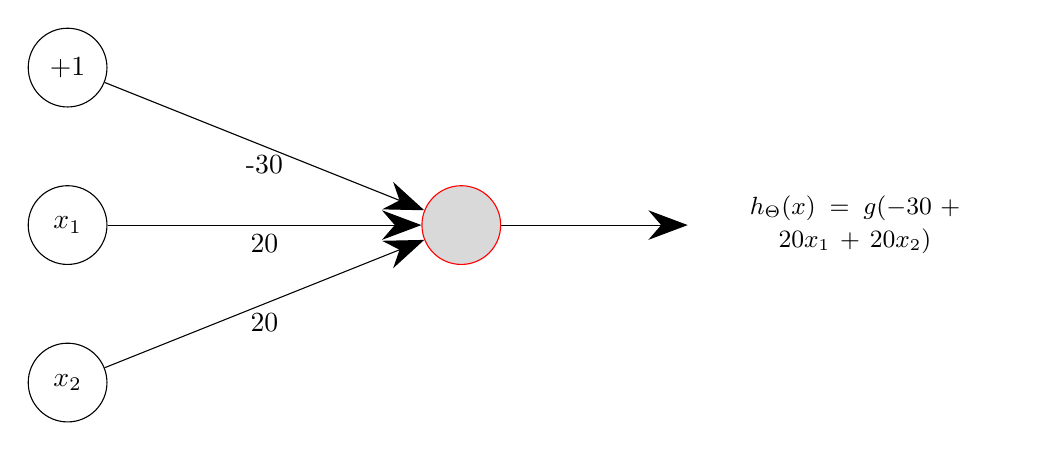
\begin{tikzpicture}[node distance=4cm]
\node (x0) [startstop] {+1};
\node (x1) [startstop, below of=x0, xshift=0cm, yshift=2cm] {$x_1$};
\node (x2) [startstop, below of=x1, xshift=0cm, yshift=2cm] {$x_2$};
\node (a1) [neuron, below of=x0, xshift=5cm, yshift=2cm] {};
\node (h) [largedetail, below of=a1, xshift=5cm, yshift=4cm] {\small{$h_{\Theta}(x) = g(-30+20x_1+20x_2)$}};
\draw [-{Stealth[length=5mm]}] (a1) -- (h);
\draw [-{Stealth[length=5mm]}] (x0) -- node[anchor=north] {-30}  (a1);
\draw [-{Stealth[length=5mm]}] (x1) -- node[anchor=north] {20} (a1);
\draw [-{Stealth[length=5mm]}] (x2) -- node[anchor=north] {20} (a1);
\end{tikzpicture}
} 
&
\begin{tabular}{cc|c|c}
\hline
\hline
$x_1$ & $x_2$ & $h_{\Theta}(x)$ & \\
\hline
0 & 0 & g(-30) $\approx 0$ & 0 \\
\hline
0 & 1 & g(-30) $\approx 0$ & 0 \\
\hline
1 & 0 & g(-30) $\approx 0$ & 0 \\
\hline
1 & 1 & g(-30) $\approx 1$ & 1 \\
\hline
\hline
\end{tabular}
\end{array}$
\end{center}
\end{figure}
This represent the logical AND function, where $h_{\Theta}(x) = 1$ if $x_1=1$ \textbf{AND} $x_2=1$.

\subsection{Logical OR function}
$x_1$ and $x_2$ $\in \{0,1\}$

\begin{figure}[H]
\begin{center}$
\begin{array}{cc}
  \resizebox {3in} {!} {
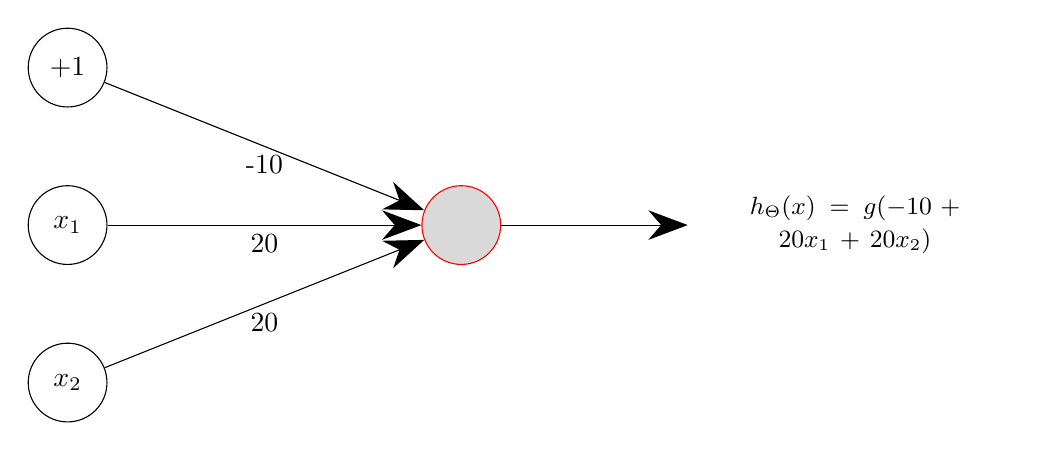
\begin{tikzpicture}[node distance=4cm]
\node (x0) [startstop] {+1};
\node (x1) [startstop, below of=x0, xshift=0cm, yshift=2cm] {$x_1$};
\node (x2) [startstop, below of=x1, xshift=0cm, yshift=2cm] {$x_2$};
\node (a1) [neuron, below of=x0, xshift=5cm, yshift=2cm] {};
\node (h) [largedetail, below of=a1, xshift=5cm, yshift=4cm] {\small{$h_{\Theta}(x) = g(-10+20x_1+20x_2)$}};
\draw [-{Stealth[length=5mm]}] (a1) -- (h);
\draw [-{Stealth[length=5mm]}] (x0) -- node[anchor=north] {-10}  (a1);
\draw [-{Stealth[length=5mm]}] (x1) -- node[anchor=north] {20} (a1);
\draw [-{Stealth[length=5mm]}] (x2) -- node[anchor=north] {20} (a1);
\end{tikzpicture}
} &
\begin{tabular}{cc|c|c}
\hline
\hline
$x_1$ & $x_2$ & $h_{\Theta}(x)$ & \\
\hline
0 & 0 & g(-10) $\approx 0$ & 0 \\
\hline
0 & 1 & g(10) $\approx 1$ & 1 \\
\hline
1 & 0 & g(10) $\approx 1$ & 1 \\
\hline
1 & 1 & g(30) $\approx 1$ & 1 \\
\hline
\hline
\end{tabular}
\end{array}$
\end{center}
\end{figure}
This represent the logical OR function, where $h_{\Theta}(x) = 1$ if $x_1=1$ \textbf{OR} $x_2=1$.

\subsection{Function Negation NOT $x_1$}
$x_1$ and $x_2$ $\in \{0,1\}$
\begin{figure}[H]
\begin{center}$
\begin{array}{cc}
  \resizebox {3in} {!} {
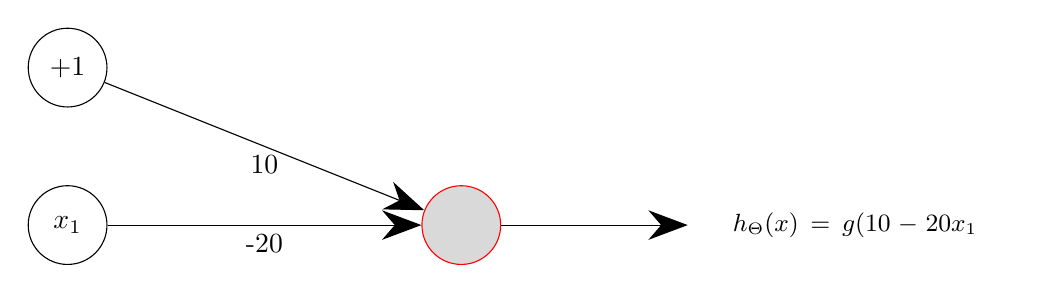
\begin{tikzpicture}[node distance=4cm]
\node (x0) [startstop] {+1};
\node (x1) [startstop, below of=x0, xshift=0cm, yshift=2cm] {$x_1$};
\node (a1) [neuron, below of=x0, xshift=5cm, yshift=2cm] {};
\node (h) [largedetail, below of=a1, xshift=5cm, yshift=4cm] {\small{$h_{\Theta}(x) = g(10-20x_1$}};
\draw [-{Stealth[length=5mm]}] (a1) -- (h);
\draw [-{Stealth[length=5mm]}] (x0) -- node[anchor=north] {10}  (a1);
\draw [-{Stealth[length=5mm]}] (x1) -- node[anchor=north] {-20} (a1);
\end{tikzpicture}
} 
&
\begin{tabular}{c|c|c}
\hline
\hline
$x_1$ & $h_{\Theta}(x)$ & \\
\hline
0 & g(10) $\approx 1$ & 1 \\
\hline
1 & g(-10) $\approx 1$ & 0 \\
\hline
\hline
\end{tabular}
\end{array}$
\end{center}
\end{figure}
This represent the logical Negate $x_1$: $y=1$ if \textbf{NOT}($x_1$)=TRUE.

\subsection{Computing $x_1$ XNOR $x_2$}
\begin{figure}[h]
\begin{center}$
\begin{array}{ccc}
 \resizebox {1.5in} {!} {
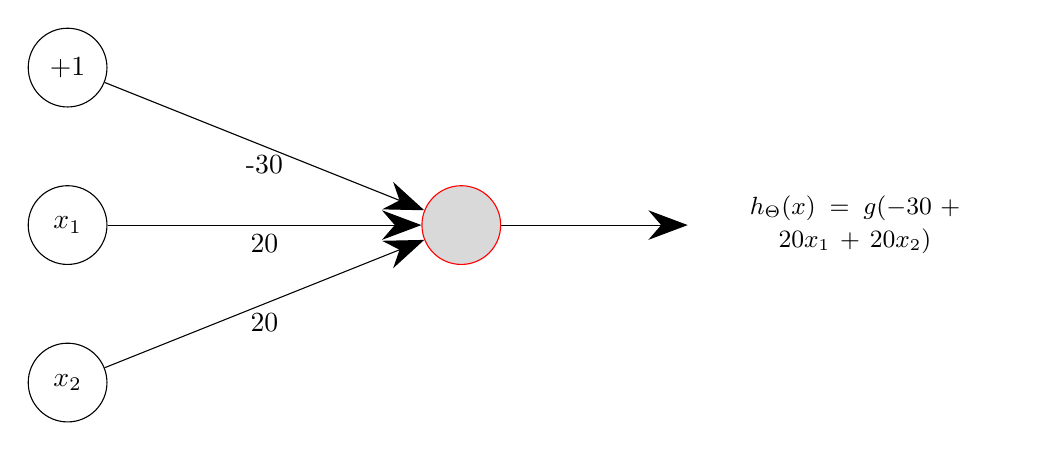
\begin{tikzpicture}[node distance=4cm]
\node (x0) [startstop] {+1};
\node (x1) [startstop, below of=x0, xshift=0cm, yshift=2cm] {$x_1$};
\node (x2) [startstop, below of=x1, xshift=0cm, yshift=2cm] {$x_2$};
\node (a1) [neuron, below of=x0, xshift=5cm, yshift=2cm] {};
\node (h) [largedetail, below of=a1, xshift=5cm, yshift=4cm] {\small{$h_{\Theta}(x) = g(-30+20x_1+20x_2)$}};
\draw [-{Stealth[length=5mm]}] (a1) -- (h);
\draw [-{Stealth[length=5mm]}] (x0) -- node[anchor=north] {-30}  (a1);
\draw [-{Stealth[length=5mm]}] (x1) -- node[anchor=north] {20} (a1);
\draw [-{Stealth[length=5mm]}] (x2) -- node[anchor=north] {20} (a1);
\end{tikzpicture}} & 
  \resizebox {1.5in} {!} {
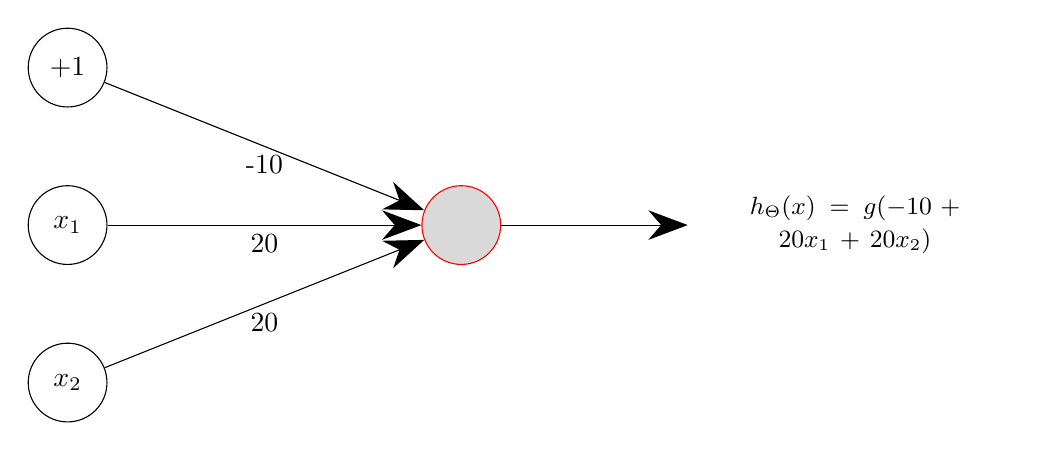
\begin{tikzpicture}[node distance=4cm]
\node (x0) [startstop] {+1};
\node (x1) [startstop, below of=x0, xshift=0cm, yshift=2cm] {$x_1$};
\node (x2) [startstop, below of=x1, xshift=0cm, yshift=2cm] {$x_2$};
\node (a1) [neuron, below of=x0, xshift=5cm, yshift=2cm] {};
\node (h) [largedetail, below of=a1, xshift=5cm, yshift=4cm] {\small{$h_{\Theta}(x) = g(-10+20x_1+20x_2)$}};
\draw [-{Stealth[length=5mm]}] (a1) -- (h);
\draw [-{Stealth[length=5mm]}] (x0) -- node[anchor=north] {-10}  (a1);
\draw [-{Stealth[length=5mm]}] (x1) -- node[anchor=north] {20} (a1);
\draw [-{Stealth[length=5mm]}] (x2) -- node[anchor=north] {20} (a1);
\end{tikzpicture}} 
&
\resizebox {1.5in} {!} {
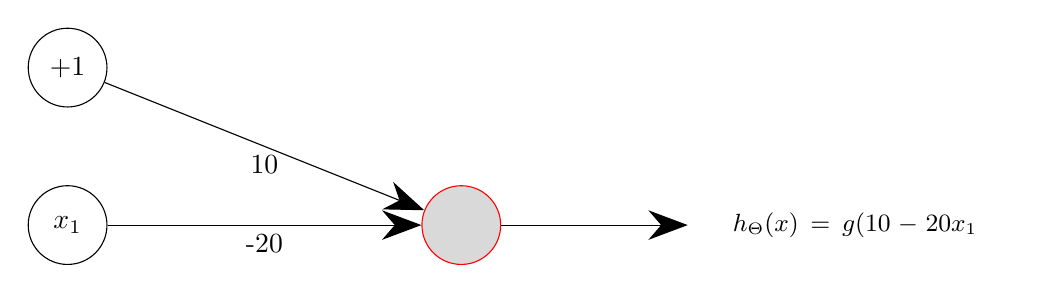
\begin{tikzpicture}[node distance=4cm]
\node (x0) [startstop] {+1};
\node (x1) [startstop, below of=x0, xshift=0cm, yshift=2cm] {$x_1$};
\node (a1) [neuron, below of=x0, xshift=5cm, yshift=2cm] {};
\node (h) [largedetail, below of=a1, xshift=5cm, yshift=4cm] {\small{$h_{\Theta}(x) = g(10-20x_1$}};
\draw [-{Stealth[length=5mm]}] (a1) -- (h);
\draw [-{Stealth[length=5mm]}] (x0) -- node[anchor=north] {10}  (a1);
\draw [-{Stealth[length=5mm]}] (x1) -- node[anchor=north] {-20} (a1);
\end{tikzpicture}}  \\ 
x_1 \mathrm{\ AND \ } x_2 & (\mathrm{NOT \ } x_1) \mathrm{\ AND\ } (\mathrm{NOT\ } x_2) & x_1 \mathrm{\ NOT\ } x_2
\end{array}$
\end{center}
\end{figure}


\begin{figure}[H]
\begin{center}$
\begin{array}{cc}
 \resizebox {3in} {!} {
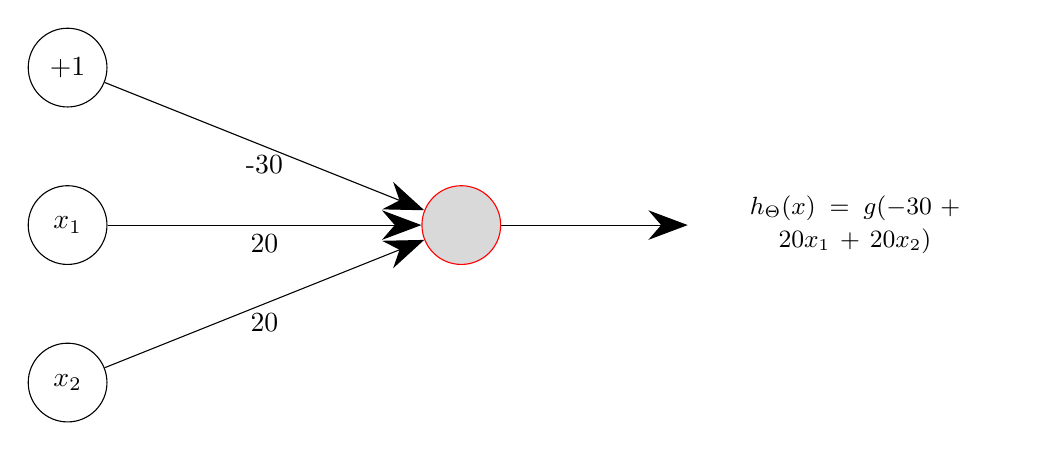
\begin{tikzpicture}[node distance=4cm]
\node (x0) [startstop] {+1};
\node (x1) [startstop, below of=x0, xshift=0cm, yshift=2cm] {$x_1$};
\node (x2) [startstop, below of=x1, xshift=0cm, yshift=2cm] {$x_2$};
\node (a1) [neuron, below of=x0, xshift=5cm, yshift=2cm] {};
\node (h) [largedetail, below of=a1, xshift=5cm, yshift=4cm] {\small{$h_{\Theta}(x) = g(-30+20x_1+20x_2)$}};
\draw [-{Stealth[length=5mm]}] (a1) -- (h);
\draw [-{Stealth[length=5mm]}] (x0) -- node[anchor=north] {-30}  (a1);
\draw [-{Stealth[length=5mm]}] (x1) -- node[anchor=north] {20} (a1);
\draw [-{Stealth[length=5mm]}] (x2) -- node[anchor=north] {20} (a1);
\end{tikzpicture}} & 
\begin{tabular}{cc|cc|c}
\hline
\hline
$x_1$ & $x_2$ & $a_1 ^{(2)}$ & $a_2 ^{(2)}$ & $h_{\Theta}(x)$\\
\hline
0 & 0 & 0 & 1 & 1 \\
0 & 1 & 0 & 0 & 0 \\
1 & 0 & 0 & 0 & 0 \\
1 & 1 & 1 & 0 & 1 \\
\hline
\hline
\end{tabular}
\end{array}$
\end{center}
\end{figure}

In summary:
\begin{itemize}
	\item $h_{\Theta}(x) = 1$ if ($x_1 = 0$ AND $x_2 = 0$) OR $(x_1 = 1$ AND $x_2 = 1)$
	\item $h_{\Theta}(x) = 0$ otherwise
\end{itemize}
This is modeled well the problem in the figure 




\subsection{ExampleII: Multiclass classification}
In this example, we define 4 classes of objects (Pedestrian, Car, Moto and Truck), and want to classify a new object within those classes. This is a multiple output unit (One-vs-all).
We will build a neuro-network with 4 output units (i.e $h_{\Theta}(x) \in \mathbb{R}^4$):
\begin{figure}[H]
        \centering
        \resizebox {0.5in} {!} {
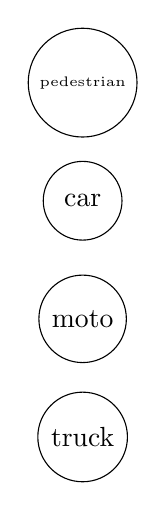
\begin{tikzpicture}[node distance=4cm]
\node (output1) [startstop] {{\tiny pedestrian}};
\node (output2) [startstop, below of=output1, xshift=0cm, yshift=2.5cm] {car};
\node (output3) [startstop, below of=output2, xshift=0cm, yshift=2.5cm] { moto};
\node (output4) [startstop, below of=output3, xshift=0cm, yshift=2.5cm] {truck};
\end{tikzpicture}
}
\end{figure}
So, we want the ouput $h_{\Theta}(x)$ to take the form: 
\begin{align*}
\begin{array}{llll}
h_{\Theta}(x) =\left[ \begin{smallmatrix} 1 \\ 0 \\ 0 \\ 0 \end{smallmatrix} \right]  & h_{\Theta}(x)=\left[ \begin{smallmatrix} 0 \\ 1 \\ 0 \\ 0 \end{smallmatrix} \right] & h_{\Theta}(x)=\left[ \begin{smallmatrix} 0 \\ 0 \\ 1 \\ 0 \end{smallmatrix} \right] & h_{\Theta}(x)=\left[ \begin{smallmatrix} 0 \\ 0 \\ 0 \\ 1 \end{smallmatrix} \right] \\
\mathrm{pedestrians} & \mathrm{car} & \mathrm{moto} & \mathrm{truck} \\
\end{array}
\end{align*}

The training set would be of the form: $(x^{(1)},y^{(1)}), (x^{(2)},y^{(2)}), ...., (x^{(m)},y^{(m)}) $, where $y^{(i)}$ is either 
\begin{align*}
\begin{array}{lllllll}
\left[\begin{smallmatrix} 1\\0\\0\\0 \end{smallmatrix} \right] & \mathrm{or} & \left[\begin{smallmatrix} 0\\1\\0\\0 \end{smallmatrix} \right] & \mathrm{or} & \left[\begin{smallmatrix} 0\\0\\1\\0 \end{smallmatrix} \right] & \mathrm{or} & \left[\begin{smallmatrix} 0\\0\\0\\1 \end{smallmatrix} \right]
\end{array}
\end{align*}

\begin{appendices}
\section{One-vs-All assignment}

\section{Answers to Quiz}
\begin{itemize}
\item Suppose you have a multi-class classification problem with 3 classes trained with a 3 layer network. Let $a_1 ^{(3)} = (h_{\Theta}(x))_1$ be the activation of the 1st output unit, and similarly  $a_2 ^{(3)} = (h_{\Theta}(x))_2$, $a_3 ^{(3)} = (h_{\Theta}(x))_3$. Then for any input $x$, it must be the case that $a_1 ^{(3)} + a_2 ^{(3)} + a_3 ^{(3)} = 1$. $\Rightarrow$ FALSE

\end{itemize}
\end{appendices}
\end{document}